\documentclass[10pt]{beamer}

%%%
% PREAMBLE FOR THIS DOC 
%%%
%https://tex.stackexchange.com/questions/68821/is-it-possible-to-create-a-latex-preamble-header
\usepackage{../preambles/beamer_preamble_for_CSCI246}



%%% TRY TO RESHOW TOC AT EACH SECTION START (with current section highlighted)
% Reference: https://tex.stackexchange.com/questions/280436/how-to-highlight-a-specific-section-in-beamer-toc
\newcommand\tocforsect[2]{%
  \begingroup
  \edef\safesection{\thesection}
  \setcounter{section}{#1}
  \tableofcontents[#2,currentsection]
  \setcounter{section}{\safesection}
  \endgroup
}



%%%
% DOCUMENT
%%%

\begin{document}






\title{Friday 08/25/2025: Theorems}
\author{CSCI 246: Discrete Structures}
\date{Textbook reference: Sec. 4, Scheinerman}


\begin{frame}
    \titlepage 
\end{frame}


\begin{frame}

\begin{mygreenbox}[title=Logistical Matters]
\begin{itemize}
\item \textbf{Announcements} - Do you get the Canvas announcements?  Preference for Canvas vs. Email?
\item \textbf{Participation grade clarification} - 10\% of your final grade is just showing up to class and doing group exercises.  I check off who's here.
\item \textbf{On group exercises} -- We may not finish the group exercises in class, but can at least get started on them.  You can try the rest as homework.  Make sure you understand the solutions before the Friday quizzes.
\item \textbf{Special circumstances for Friday 08/29} -- Office hours from 9am-12pm.  Guest instructor: Kunal Das, Ph.D.
\end{itemize}

\end{mygreenbox}

\vfill 


\begin{myyellowbox}[title=Today's Agenda]
\begin{itemize}
	\item Logistics/practice quiz ($\approx$ 10 mins)
	\item Mini lecture ($\approx$ 15 mins)
	\item Group exercises ($\approx$ 15 mins) and review ($\approx$ 10 mins)
\end{itemize}


\end{myyellowbox}
\vfill 

\end{frame}


\begin{frame}{Practice Quiz}

Replace each $\red{?}$ with a checkmark \greencheck if the combination of truth values for propositions A and B is \textit{possible} under the given logical connective.  Replace it with a \redx if the combination is \textit{impossible}.

\begin{table}
\centering
\begin{tabular}{cc|ccc}
\multicolumn{2}{c}{\textbf{Propositions}} & \multicolumn{3}{c}{\textbf{Logical Connectives}} \\
A  & B & if A then B & if B then A & A if and only if B \\
\hline 
T & T & \red{?} & \red{?} & \red{?}\\
T & F &\red{?}  & \red{?} & \red{?} \\
F & T & \red{?} & \red{?} & \red{?} \\
F & F & \red{?} &\red{?}  & \red{?}
\end{tabular}
\end{table}

\pause 
\begin{center}
\bluetextbox{The goal of today's slides is to clarify the solution.}	
\end{center}

\end{frame}


%%%% Section
\begin{frame}[standout]
If A, then B
\end{frame}


\begin{frame}{If A, then B: Truth Table}
\label{slide:truth_table_for_if_A_then_B}
Given two propositions $A$ and $B$, the statement \qq{If A, then B} (that is, the property $A  \implies B$) holds whenever following \qq{truth table} applies:

\begin{center}
\begin{tabular}{cc|c}
A & B & $\overbrace{A \implies B}^{\text{If A, then B}}$ \\
\hline 
T & T & \green{T} \\
T & F & \red{F} \\
F & T & \green{T}  \\
F & F & \green{T}  \\
\end{tabular}
\end{center}
\pause  
\vfill 
\colorbox{blue!30}{\textbf{Summary.}} If A is True, B \alert{must} be True. 
\pause  
\vfill  
\colorbox{yellow!30}{\textbf{Remark.}}  If A is False, then no restrictions are placed on B.
\pause  
\vfill
\colorbox{green!30}{\textbf{Example.}} Let $A$ = \texttt{This person lives in Bozeman}, $B$ = \texttt{This person lives in Montana}.  Here, $A \implies B$.  (Check this against the truth table.)
\end{frame}



\begin{frame}{If A, then B: Set Theoretic Perspective}
Let \red{$A$} = \texttt{This person lives in Bozeman} and \blue{$B$} = \texttt{This person lives in Montana}.   Then $A \implies B$!

\begin{columns}[T] % align columns at the top

% Left column: TikZ diagram
\begin{column}{0.6\textwidth}
\begin{center}
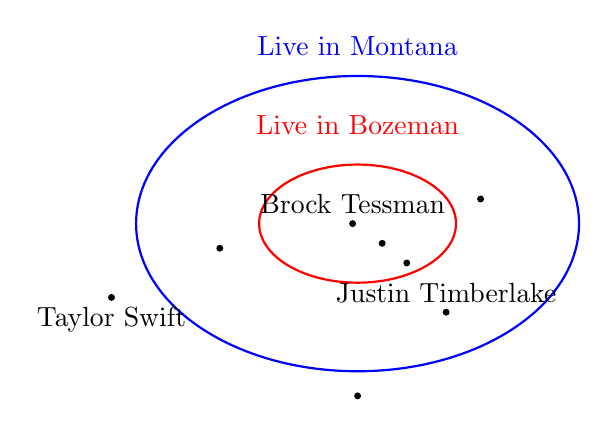
\begin{tikzpicture}[scale=0.625]
% Draw outer shape B
\draw[thick, blue] (0,0) ellipse (4.5cm and 3cm) node[above=2cm] {Live in Montana};

% Draw inner shape A
\draw[thick, red] (0,0) ellipse (2cm and 1.2cm) node[above=1cm] {Live in Bozeman};

% Points inside A
\fill (0.5,-0.4) circle (2pt);
\fill (-0.1,0.0) circle (2pt);
\fill (1,-0.8) circle (2pt);
\node[above] at (-0.1,0.0) {Brock Tessman}; % labeled point inside A

% Points inside B but not A
\fill (2.5,0.5) circle (2pt);
\fill (-2.8,-0.5) circle (2pt);
\fill (1.8,-1.8) circle (2pt);
\node[above] at (1.8,-1.8) {Justin Timberlake}; % labeled point in B but not A

% Points outside B
\fill (-5,-1.5) circle (2pt);
\fill (0,-3.5) circle (2pt);
\node[below] at  (-5,-1.5) {Taylor Swift}; % labeled point outside B

\end{tikzpicture}
\end{center}
\end{column}

% Right column: Justin Timberlake picture
\begin{column}{0.4\textwidth}
\begin{center}

\includegraphics[width=\textwidth]{images/jt}	
\end{center}
\end{column}
\end{columns}


\vfill 
\pause 

 \vfill 
 \pause 
\vfill  
\colorbox{yellow!30}{\textbf{Set theoretic perspective.}}  You can think about $A \implies B$ as \qq{the set of things satisfying property $A$ is contained within the set of things satisfying property $B$.}

\end{frame}


% Now we install the new template for the following frames:
{\usebackgroundtemplate{%
  
\includegraphics[width=\paperwidth,height=\paperheight]{images/flying_elephant}} 
\begin{frame}
\centering 
\Large \color{black} \textbf{Poll: True or False?} Every elephant flying with polka-dotted balloons above Bozeman is smoking a cigar. \color{black}
\vfill \vfill \vfill \vfill 
\end{frame}
}


\begin{frame}{Vacuous Truths}


\begin{mygreenbox}[title=Solution to poll]
Let $A$ = \texttt{this is an elephant flying with polka-dotted balloons above Bozeman} and $B$ = \texttt{this is smoking a cigar}.  Then $A$ is always False. So $A \implies B$ is \alert{TRUE!!!} This is called a \textbf{vacuous truth.}  Per Scheinerman, these statements are true \qq{because they have no exceptions.}
\end{mygreenbox}

\pause  
\vfill 

\begin{myyellowbox}[title=Reference material]
Given two propositions $A$ and $B$, the statement \qq{If A, then B} ($A  \implies B$) holds whenever following \qq{truth table} applies:

\begin{center}
\begin{tabular}{cc|c}
A & B & $\overbrace{A \implies B}^{\text{If A, then B}}$ \\
\hline 
T & T & \green{T} \\
T & F & \red{F} \\
F & T & \green{T}  \\
F & F & \green{T}  \\
\end{tabular}
\end{center}
\end{myyellowbox}

\end{frame}


\begin{frame}{If A, then B: Other jargon}

Some other terminology which means the same thing:
\begin{itemize}
\item A implies B
\item A is sufficient for B
\item B is necessary for A (A "only if" B)
\end{itemize}
 
	
\end{frame}


%%%% Section
\begin{frame}[standout]
A if and only if B
\end{frame}


\begin{frame}

%The biconditional \texttt{A if and only if B} (written $A \iff B$) can be defined as $(A \implies B) \, \texttt{and} \, (B \implies A)$.

\vfill \pause 
\begin{myredbox}[title=\textit{If and only if} statements: Main Idea]

\[ \explaintermbrace{A if and only if B}{A \iff B} \quad \text{means} \quad \explaintermbrace{A only if B}{(A \implies B)} \; \texttt{and} \; \explaintermbrace{A if B}{(A  \impliedby B)} \] 
\end{myredbox}

\end{frame}


\begin{frame}{A if and only if B: Details}
\footnotesize
 The truth table for the ``\texttt{and}" operator (also written $\land$) is given by  
\begin{center}
\begin{tabular}{cc|c}
\multicolumn{2}{c}{\textbf{Original propositions}} & \multicolumn{1}{c}{\textbf{New proposition}} \\
X & Y & $X \land Y$ \\
\hline 
T & T & T \\
T & F & F \\
F & T & F  \\
F & F & F  \\
\end{tabular}
\end{center}
\pause 
Now we apply the $\land$ operator to the results of the $\implies$ and $\impliedby$ operators.
 
\begin{table}
\centering
\begin{tabular}{cc|ccc}
\multicolumn{2}{c}{\textbf{Orig. props.}} & \multicolumn{3}{c}{\textbf{New props.}} \\
A & B & $\overbrace{A \implies B}^{X}$  & $\overbrace{B \implies A}^{Y}$& $\overbrace{(A \implies B) \land  (B \implies A)}^{X \land Y}$ \\
\hline 
T & T & \green{T}  & \green{T} & \green{T}\\
T & F & \red{F} & \green{T} &  \red{F}  \\
F & T & \green{T}  &  \red{F}  &  \red{F}  \\
F & F & \green{T} & \green{T} & \green{T}
\end{tabular}
\end{table}

\end{frame}

\begin{frame}{A if and only if B: Truth Table}

Given two propositions $A$ and $B$, the statement \qq{A if and only if B} (that is, the property $A  \iff B$) holds whenever following \qq{truth table} applies:

\begin{center}
\begin{tabular}{cc|c}
A & B & $\overbrace{A \iff B}^{\text{A if and only if B}}$ \\
\hline 
T & T & \green{T} \\
T & F & \red{F} \\
F & T & \red{F}  \\
F & F & \green{T}  \\
\end{tabular}
\end{center}
\pause  
\vfill 
\colorbox{blue!30}{\textbf{Summary.}} A and B are \underline{both} True or \underline{both} False.
\pause  
\vfill  
\colorbox{green!30}{\textbf{Example.}} Let $A$ = \texttt{Labor Day is in this month}, $B$ = \texttt{This month is September}.  Here, $A \iff B$.  (Check this against the truth table.)
\end{frame}


\begin{frame}{A if and only if B: Set theoretic perspective}
Let \red{$A$} = \texttt{Labor Day is in this month} and \blue{$B$} = \texttt{This month is September}.   Then $A \iff B$!

\begin{center}
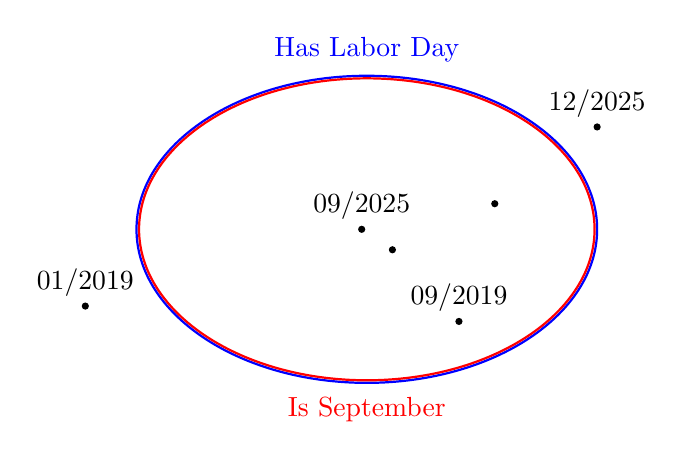
\begin{tikzpicture}[scale=0.65]
% Draw outer shape B
\draw[thick, blue] (0,0) ellipse (4.5cm and 3cm) node[above=2cm] {Has Labor Day};

% Draw inner shape A
\draw[thick, red] (0,0) ellipse (4.45cm and 2.95cm) node[below=2cm] {Is September};

% Points inside A and B
\fill (0.5,-0.4) circle (2pt);
\fill (2.5,0.5) circle (2pt);
\fill (-0.1,0.0) circle (2pt);
\fill (1.8,-1.8) circle (2pt);
\node[above] at (-0.1,0.0) {09/2025}; % labeled point inside A
\node[above] at (1.8,-1.8) {09/2019}; % labeled point in B but not A

% Points outside B
\fill (4.5,2) circle (2pt);
\fill (-5.5,-1.5) circle (2pt);
\node[above] at (4.5,2) {12/2025}; % labeled point outside B
\node[above] at (-5.5,-1.5) {01/2019}; % labeled point outside B

\end{tikzpicture}
\end{center}
\vfill 
\pause 

 \vfill 
 \pause 
\vfill  
\colorbox{yellow!30}{\textbf{Set theoretic perspective.}}  You can think about $A \iff B$ as \qq{the set of things satisfying property $A$ is identical to the set of things satisfying property $B$.}

\end{frame}



%%%% Section
\begin{frame}[standout]
Solution to practice quiz
\end{frame}


\begin{frame}{Solution to practice quiz}
\small 
\begin{table}
\centering
\begin{tabular}{cc|ccc}
\multicolumn{2}{c}{} & \multicolumn{3}{c}{} \\
A  & B & if A then B & if B then A & A if and only if B \\
\hline 
T & T & \green{T}  & \green{T} & \green{T}\\
T & F & \red{F} & \green{T} &  \red{F}  \\
F & T & \green{T}  &  \red{F}  &  \red{F}  \\
F & F & \green{T} & \green{T} & \green{T}
\end{tabular}
\end{table}
\end{frame}




%%%% Section
\begin{frame}[standout]
The Big Picture: \\
Propositional Logic
\end{frame}


\begin{frame}{Propositional logic}
\label{slide:prop_logic}
\small 
\begin{table}
\centering
\begin{tabular}{cc|ccc}
\multicolumn{2}{c}{\textbf{Original propositions}} & \multicolumn{3}{c}{\textbf{New propositions}} \\
A  & B & if A then B & if B then A & A if and only if B \\
\hline 
T & T & \green{T}  & \green{T} & \green{T}\\
T & F & \red{F} & \green{T} &  \red{F}  \\
F & T & \green{T}  &  \red{F}  &  \red{F}  \\
F & F & \green{T} & \green{T} & \green{T}
\end{tabular}
\end{table}
\pause 
\vfill 
\begin{itemize}
\item The column headings show 3 new propositions, formed from the original propositions by \textbf{logical connectives}. \pause 
\item Each logical connective can be thought of as a \textbf{function} or mapping $\set{T,F} \times \set{T,F} \to \set{T,F}$.  \pause 
\item Besides \texttt{if-then} and \texttt{if-and-only-if}, there are other logical connectives (\texttt{and, or, xor}, etc.), some of which were discussed in the text. \pause 
\item The study of how to combine and change propositions under logical connectives to form more complex propositions is called \textbf{propositional logic}. 
\end{itemize}

\vfill \pause 
\colorbox{yellow!30}{\textbf{Terminology.}} The first two columns combined with one remaining column gives the \alert{\textbf{truth table}} for that logical connective. 
\end{frame}


\begin{frame}[standout]
Group exercises
\end{frame}

\begin{frame}{Random group assignments}
\footnotesize 
\vfill 
\begin{columns}
\begin{column}{0.33\textwidth}
Aaron Christensen: 1 \\ 
Aidan Sinclair: 6 \\ 
Brendan Kelly: 9 \\ 
Buggy Garza: 6 \\ 
Cedric Jefferson: 3 \\ 
Conner Brost: 7 \\ 
Connor Graville: 4 \\ 
David Knauert: 2 \\ 
David Oswald: 16 \\ 
Elias Martin: 9 \\ 
Ericson O'Guinn: 3 \\ 
Erik Halverson: 15 \\ 
Francis Bush: 6 \\ 
Garrett Miller: 14 \\ 
George Cutler: 7 \\ 
Georgia Franks: 10 \\ 
Gregor Schmidt: 16 \\\end{column}
\begin{column}{0.33\textwidth}
Hakyla Riggs: 8 \\ 
Izayah Abayomi: 1 \\ 
Jacob Ketola: 11 \\ 
Jacob Ruiz: 13 \\ 
Jaden Hampton: 5 \\ 
Jeremy Ness: 7 \\ 
Jonah Day: 8 \\ 
Karter Gress: 16 \\ 
Kyle Hoerner: 17 \\ 
Landry Clarke: 8 \\ 
Leon BirdHat: 4 \\ 
Lillian Ziegler: 17 \\ 
Matthew Rau: 12 \\ 
Micah Miller: 15 \\ 
Michael Pitman: 1 \\ 
Nathan Campbell: 2 \\\end{column}
\begin{column}{0.33\textwidth}
Nathan Hooley: 10 \\ 
Nicholas Rugani: 2 \\ 
Noah Andersson: 13 \\ 
Olivia Greuter: 4 \\ 
Peter Van Vleet: 14 \\ 
Pierce Dotson: 11 \\ 
Quinn Carlson: 10 \\ 
Ridley Christoferson: 12 \\ 
Riley Smith: 5 \\ 
Sierra Holleman: 11 \\ 
Tanner Gramps: 9 \\ 
Timothy True: 15 \\ 
Titus Sykes: 5 \\ 
Trey Randall: 12 \\ 
William Grant: 13 \\ 
William Sheldon: 14 \\ 
Zachary Reller: 3 \\\end{column}
\end{columns}
\vfill \vfill \vfill
\textbf{Note:} If your name is not here, please come see me so I can get you on the roster. 
\end{frame}



\begin{frame}{Group exercises}
\small 
\begin{enumerate}
 % Scheinerman
	\item It is a common mistake to confuse the following two statements (i) If A, then B and (ii) If B, then A. Find two conditions A and B such that statement (i) is true but statement (ii) is false. Then find two conditions A and B such that both statements are true. 
 % Scheinerman
	\item Consider these two statements: (i) If A, then B, (ii) If (not B), then (not A).  Under what circumstances are these statements true?  When are they false? Explain whether these statements are identical or not. \alert{[Note: (ii) is called the \textbf{contrapositive} of (i).]}
 % Norman Swartz
	\item (Challenge problem, from philosopher Norman Swartz.)  Is the following statement true or false, and why? \textit{A's-being-a-necessary-condition-for-B is both a necessary and sufficient condition for B's-being-a-sufficient-condition-for-A.}
\end{enumerate}
	
\end{frame}


\begin{frame}{Question 1: Solution}
$A \implies B$ but $B \centernot\implies A$: \\
A = I lived in Los Angeles \\
B = I lived in California. \\
\vfill 
$A \iff B$: \\
A = Valentine's Day is this month \\
B = This month is February. 
\end{frame}



\begin{frame}{Question 2: Solution}
\footnotesize
Recall from Slide \ref{slide:truth_table_for_if_A_then_B} that the truth table for the $\implies$ operator is given by  
\begin{center}
\begin{tabular}{cc|c}
X & Y & $\overbrace{X \implies Y}^{\text{If X, then Y}}$ \\
\hline 
T & T & T \\
T & F & F \\
F & T & T  \\
F & F & T  \\
\end{tabular}
\end{center}

Now we apply the $\implies$ operator to the results of the "\texttt{not}" operator (also written $\lnot$).
 
\begin{table}
\centering
\begin{tabular}{cc|ccc}
\multicolumn{2}{c}{\textbf{Orig. props.}} & \multicolumn{3}{c}{\textbf{New props.}} \\
A & B & $\overbrace{\lnot A}^{Y}$  & $\overbrace{\lnot B}^{X}$& $\overbrace{\lnot B \implies \lnot A}^{X \implies Y}$ \\
\hline 
T & T & \red{F}  & \red{F} & \green{T}\\
T & F & \red{F} & \green{T} &  \red{F}  \\
F & T & \green{T}  &  \red{F}  &  \green{T}  \\
F & F & \green{T} & \green{T} & \green{T}
\end{tabular}
\end{table}
%
Note that $\lnot B \implies \lnot A$ gives the same results as $A \implies B$ as on Slide \ref{slide:truth_table_for_if_A_then_B}.
\vfill 
\pause 
\bluetextbox{Remark: We've shown that a proposition is logically equivalent to its contrapositive.  So what?  Sometimes it's easier to verify the contrapositive version.} 
\end{frame}

\begin{frame}{Question 3: Solution}
The simplest way to see this is as follows:
\begin{itemize}
\item A's-being-a-necessary-condition-for-B can be expressed as $B \implies A$.
\item B's-being-a-sufficient-condition-for-A can be expressed as $B \implies A$. 
\item In other words, both propositions are the same: $B \implies A$. And a proposition is always necessary and sufficient for itself.  
\end{itemize}

\end{frame}


\end{document}
